%!TEX root = ../template.tex
%%%%%%%%%%%%%%%%%%%%%%%%%%%%%%%%%%%%%%%%%%%%%%%%%%%%%%%%%%%%%%%%%%%%
%% chapter4.tex
%% NOVA thesis document file
%%
%% Chapter with lots of dummy text
%%%%%%%%%%%%%%%%%%%%%%%%%%%%%%%%%%%%%%%%%%%%%%%%%%%%%%%%%%%%%%%%%%%%

\typeout{NT FILE chapter4.tex}%

\chapter{Implementation}
\label{cha:implementation}

\paragraph{}In this chapter, the implementation of the different modules 
and components mentioned in the previous chapter will be described, 
as well as their process of creation and integration into the 
full system.

\section{Software}
\label{sec:software}
\paragraph{}Since this system is composed of several different components that need 
to run independantly, the software used will need to be robust enough to account for 
each component's requirements, and for this task there the \gls{ROS} framework is used.
There are two versions of this framework, \gls{ROS} and \gls{ROS2}, the latter being the 
most recent version, which is the one to be used in this project.

\subsection{ROS2}
\label{subsec:ros2}
\paragraph{}The \gls{ROS2} framework is a set of software libraries and tools that 
help developers create robotic applications. It is provides a set of solutions to various 
problems, such as parallelism, communication, modularity, and hardware abstraction.

It works by creating a network of nodes (python or c++ programs) that can communicate with each other 
using a publish-subscribe model and a service-client model. The former is a broadcasting 
model where a node can publish messages to a specific topic, and any other 
program can subscribe to that same topic and receive those messages and usse them using callbacks. 
The latter is a request-response model where a specific node is the server and other 
nodes can call it to request a specific service, which helps with modularity 
as each node can have its own specific task and be developed independently. When it comes to 
the hardware abstraction, since the software is wildly used in the robotics community 
it already has a lot of packages and libraries that can be used to interpret data form 
sensors, control actuators, and even simulate the robot in a virtual environment.


\subsection{NAV2}
\label{subsec:navigation2}
\paragraph{}The \gls{NAV2} stack is a set of packages that provide a framework for autonomous navigation. 
It is built on top of \gls{ROS2} and provides a set of tools for coordinating the different components of 
the navigation system.
\begin{figure}[h]
    \centering
    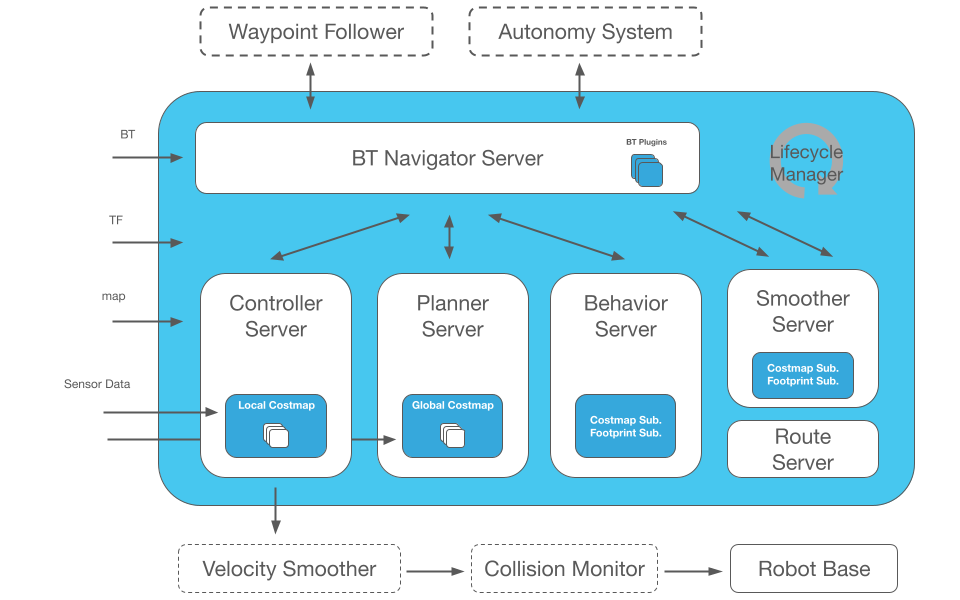
\includegraphics[width=0.8\textwidth]{nav2_architecture.png}
    \caption{NAV2 stack architecture \cite{nav2_architecture}}
    \label{fig:nav2_stack}
\end{figure}

In figure \ref{fig:nav2_stack} we can see the different components of the \gls{NAV2} stack as well as their 
relations with one another. Firstly, lets define the inputs to the diagram. The BT is the Behaviour tree 
which is an xml file that defines the robot's behaviour, the TF a collection of transforms that define each 
robot link to one another, the map is a 2D map representing the environment, and the sensor data is 
the data collected by the robot's sensors. Secondly, some essencial elements are also the global and local 
costmaps, which are 2D maps that instead of having binary values for if there's an obstacle or not, have 
have costs for each cell that represent the difficulty of traversing that cell, the Global costmap 
has the map origin as a reference for the robot's position, while the local costmap is centered around 
the robot's position. Having these concepts defined, we can now explain the different components of 
the \gls{NAV2} stack. The BT navigator server is the main component of the navigation as it manages 
and interacts with all the other servers to achieve a robust navigation solution. The Controller server, 
given the global path and the local costmap, is responsible for generating velocity commands 
for the robot to follow the path, it does this by using a controller plugin that can be custom made or 
one of the many already available in the stack. The Planner server is responsible for, given the 
global costmap and the robot's position, generating a global path to the goal, it does this by also 
using a plugin. The Behaviour server is given both costmaps and decides what action the robot should take 
in a given moment. Lastly, the Lifecycle manager, this node is responsible for managing the lifecycle of all 
the other nodes in the navigation stack, ensuring that they are properly initialized, configured, and shut 
down as needed. These are the main components as the other servers are not essential for understanding 
the navigation and overall architecture of the system.





\section{Environment}
\label{subsec:environment}
\paragraph{}For development purposes, a virtual environment is used to develop the navigation software 
and test it without the need for a physical robot. This environment can be created using Gazebo, a 
robotics simulator that is compatible with \gls{ROS2}, and it allows the user to create a world in xml format, specifying 
the different physical properties of the environment as well as the structures and objects inside it.

Since the robot will be operating in an agricultural environment, the world created for 
the simulation would have to reflect that, so a simple world was created with five 
corridors with traffic bariers on each side (to simulate trees or crops) and some additional 
obstacles to make for a more complex environment.
\begin{figure}[H]
    \centering
    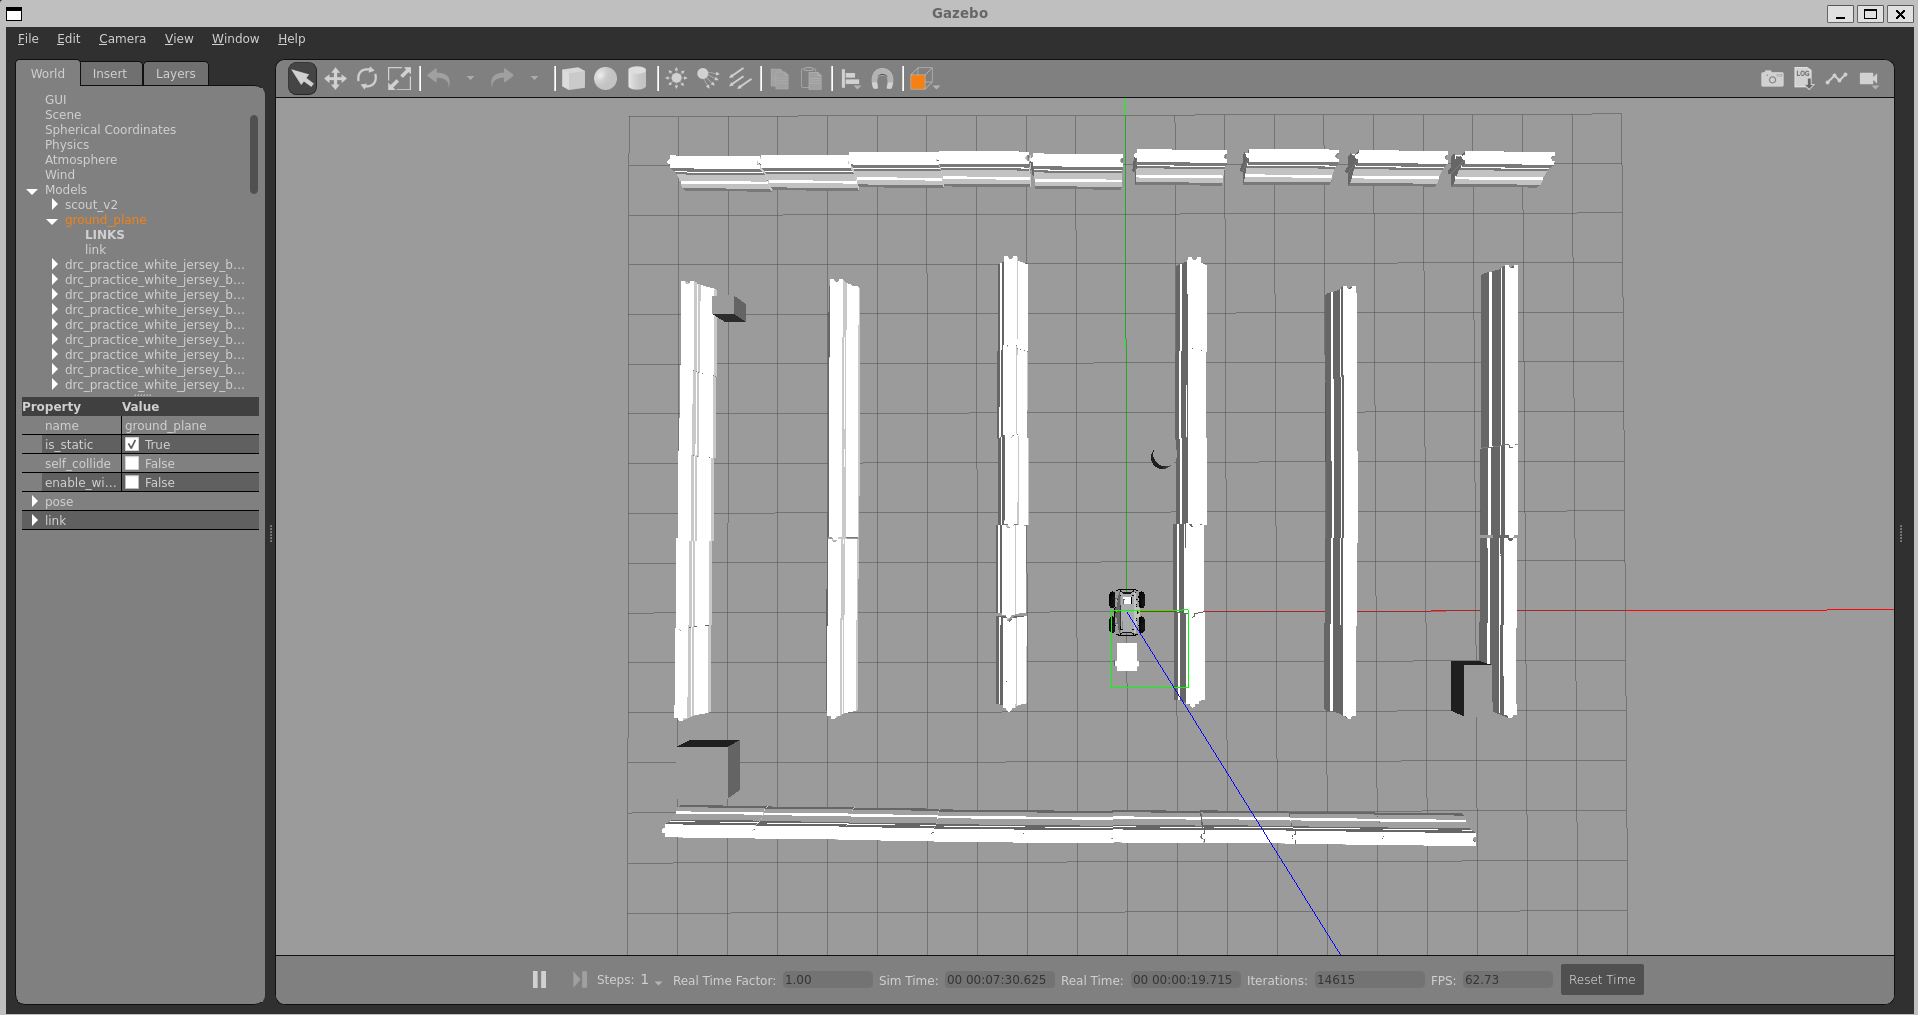
\includegraphics[width=0.9\textwidth]{gazeboworld.png}
    \caption{Gazebo world used for simulation.}
    \label{fig:gazebo_world}
\end{figure}

Having the world isn't enough to have a fully autonomous robot, a map 
of the world is also required for the localization and navigation components to work. 
this map can be created using the \gls{SLAM} algorithm, as mentioned in the previous chapter \ref{sec:slam}. 
Since the \gls{NAV2} stack already has a package that implements the \gls{SLAM} algorithm, all it needs is to 
have the robot's model and sensors running in the environment, and it will create a map.
The robot model used in this work is fortunately made available by its manufacturers 
so it can be used in the simulation directly, and the sensors are simulated using their 
Gazebo plugins, which allow the user to specify the sensor's properties, such as range, resolution, and noise.
\clearpage
\begin{figure}
    \centering
    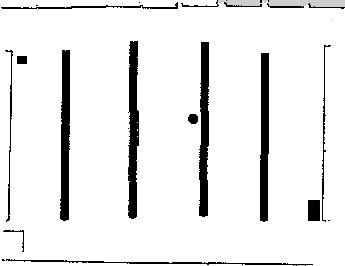
\includegraphics[width=0.7\textwidth]{wall_map.png}
    \caption{Map created using the SLAM Package in the Gazebo Simulation. White space is non-occupied space, black are obstacles and grey is undiscovered space.}
    \label{fig:slam_map}
\end{figure}

The map shown in figure \ref{fig:slam_map} is the result of mapping the simulated environment, 
however, since this work aims to have an operational prototype, two other maps were created 
in real world locations, one in a concealed room and another in a corridor with a few obstacles to simulate the rows 
of crops. 

These last two maps, due to being created in real world locations, can't be 
simulated in gazebo, so the hardware interface for the robot and its sensors 
would need to be implemented in order to comunicate within the \gls{ROS2} framework. 
Fortunately the necessary packages were all provided by the manufactures \cite{ScoutRepo, RoboSense} and only needed a few adjustments to 
be completely integrated witin the system. Since the LIDAR used is a 3D LIDAR, the output 
of the sensor is a point cloud, however, the \gls{SLAM} package used outputs 2D Maps and would need a 
Laser Scan to be used. To overcome this a \gls{ROS2} package was used (Pointcloud to Laser Scan) that 
given the distance and angles that need to be covered, converts a point cloud into a laser scan, 
allowing for the \gls{SLAM} package to work as intended.
\begin{figure}[H]
    \centering
    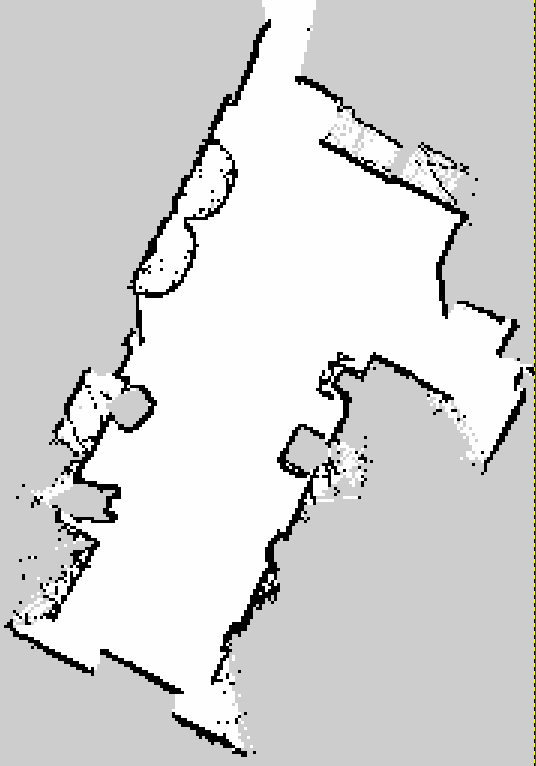
\includegraphics[width=0.90\textwidth]{basement.png}
    \caption{Map of the concealed room.}
    \label{fig:basement_map}
\end{figure}
\begin{figure}[H]
    \centering
    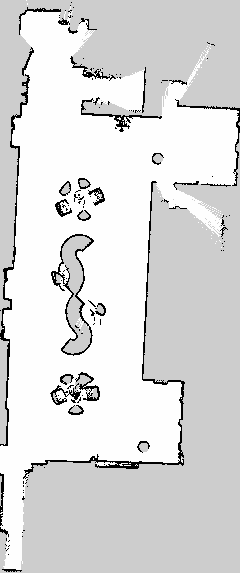
\includegraphics[width=0.65\textwidth]{corridor_map.png}
    \caption{Map of the corridor.}
    \label{fig:corridor_map}
\end{figure}

To visualize the robot in these maps as well as all the different data that is deemed relevant, a software called 
Rviz2 is used. This software allows the user to select the various \gls{ROS2} topics that are being published 
by the running nodes and visualize them in a 3D environment, which is very useful for debugging and testing purposes.
\begin{figure}[H]
    \centering
    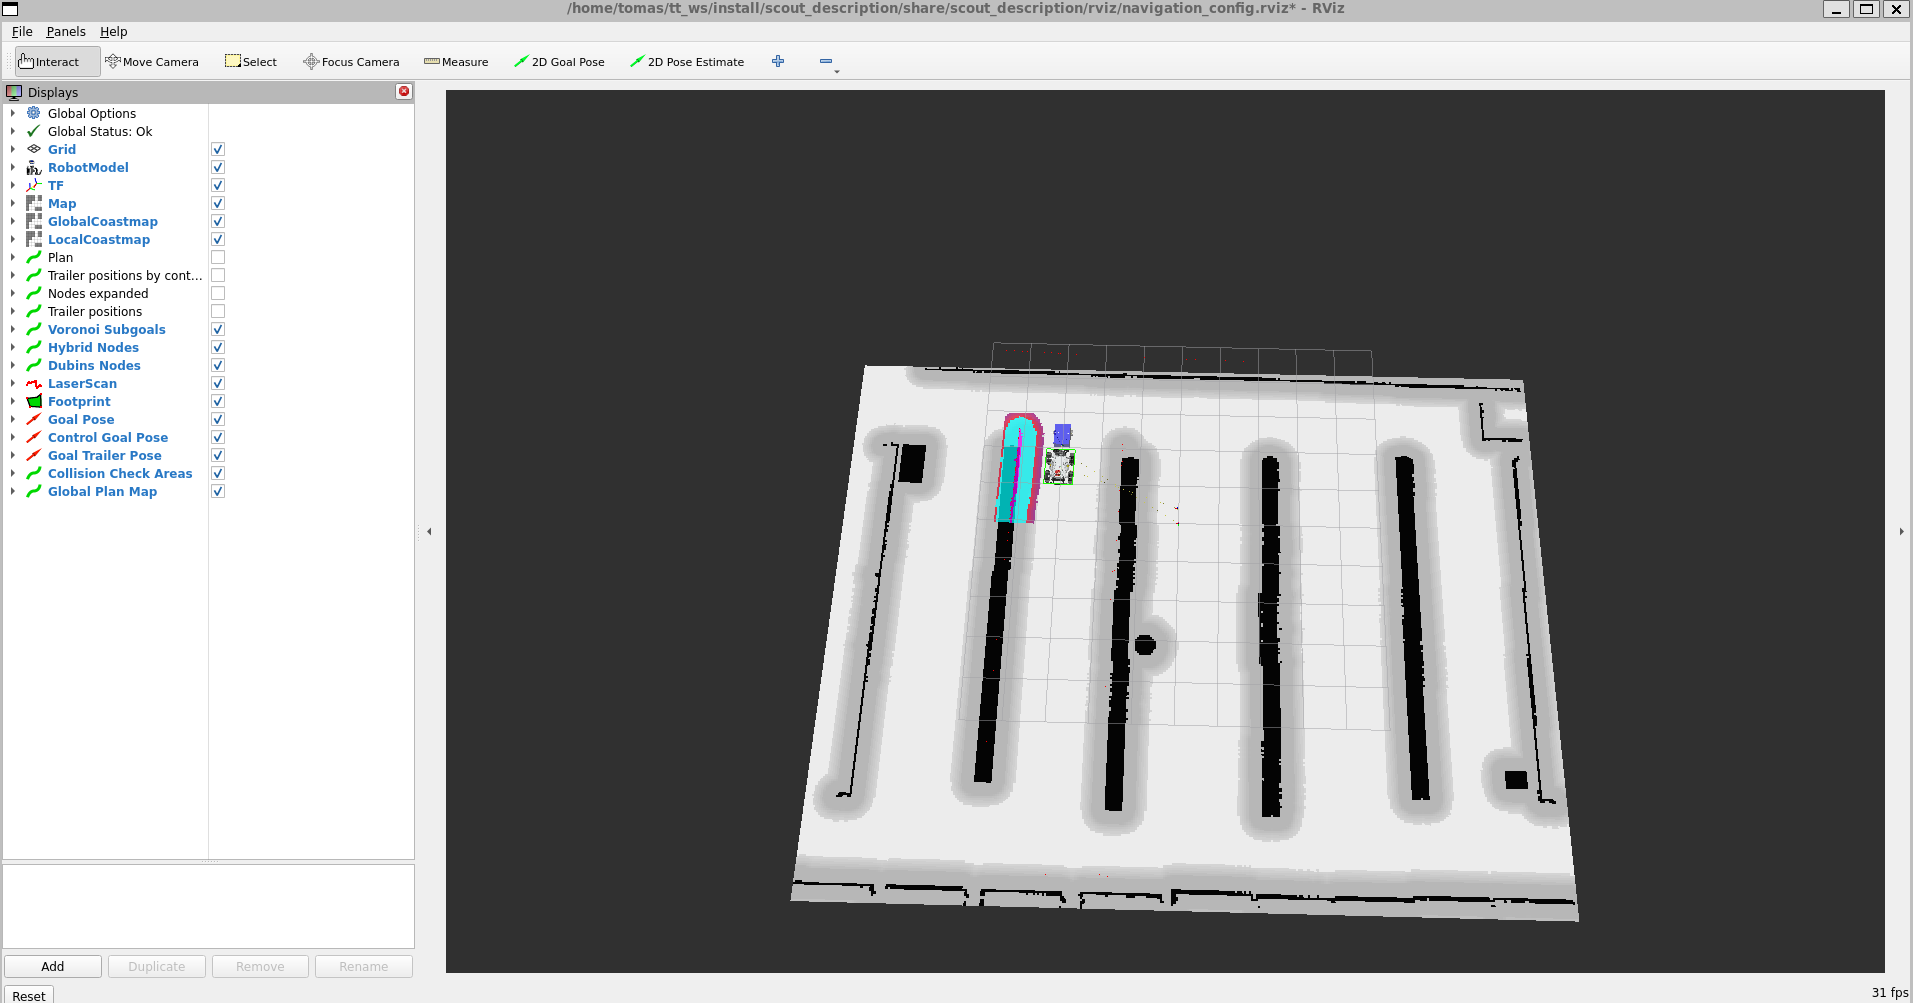
\includegraphics[width=0.9\textwidth]{Rviz2viz.png}
    \caption{Rviz2 visualization of the robot in the simulated environment.}
    \label{fig:rviz2_visualization}
\end{figure}

The figure \ref{fig:rviz2_visualization} shows, at the left, the different data provided by the developed system and, above it the 
navigation tools like estimatin the robot's initial position and goal generation. These last two tools can be used manually 
in Rviz2 or be published by a custom node if the user requires it.

\section{Planning algorithm}
\label{sec:planning_algorithm}

\paragraph{}As explained in the previous chapter \ref{sec:planner1}, 
the planner is devided into three main components, the Voronoi Graph, the Dubins Path and the Hybrid A* recovery algorithm.

\subsection{Voronoi Graph}
\label{subsec:voronoi_graph}

\paragraph{}The main function of the Voronoi Graph is to create a set of points in space that can be searched for a  
simple path to the goal using an A* search. Due to the nature of calculating a Voronoi Graph, it can be very computationally 
expensive, so the algorithm is ran offline, when the environment is mapped, and the resulting graph is saved to a 
file for the online planner to use. To create this graph, a Ros2 python node was created that executes a script with 
the previous behaviour.

The algorithm first works by creating black and white image containing the edges of the obstacles and grouping them 
into a single column of points which are then used to calculate the Voronoi Graph using the 
Scipy library \cite{Scipy}. 
This graph is then filtered to remove points that are inside the obstacles and remove points that are too close to each other. Points can be created inside the obstacles 
because of their width, so the algorithm considers it available space. To filter them, they are 
place on the original map, and  if they're not in white space, they're removed.
\begin{figure}[h]
    \centering
    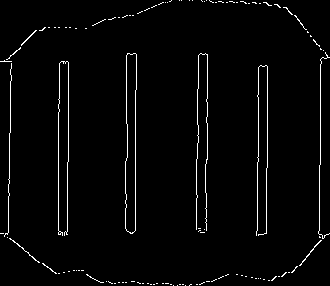
\includegraphics[width=0.7\textwidth]{edges_map_V20.png}
    \caption{Image with the obstacle edges.}
    \label{fig:voronoi_edges}
\end{figure}
\begin{figure}[h]
    \centering
    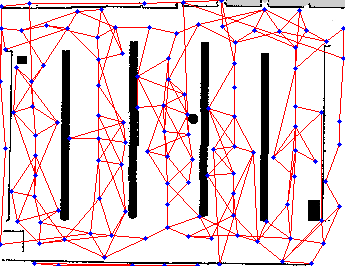
\includegraphics[width=0.7\textwidth]{voronoi_graph_V100.png}
    \caption{First Voronoi Graph created for the environment in figure \ref{fig:gazebo_world}.}
    \label{fig:voronoi_graph1}
\end{figure}

It is possible to verify that the graph isn't exacly perfect, as it doesn't 
show the usual behaviour of a Voronoi Graph with straight lines equidistant to the 
obstacles, however, this is due to the jagged nature of the edges of the obstacles, creating 
several equidistant points. Dispite thos, this graph is pourly dense in some 
areas compared to others, so a second iteration is made to correct this.
\begin{figure}[h]
    \centering
    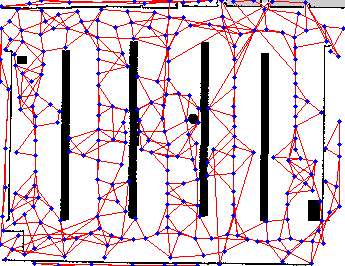
\includegraphics[width=0.8\textwidth]{voronoi_graph_V101.png}
    \caption{Second Voronoi Graph created for the environment in figure \ref{fig:gazebo_world}.}
    \label{fig:voronoi_graph2}
\end{figure}

An then finalized with a third iteration that now resembles a more 
traditional Voronoi Graph.
\begin{figure}[h]
    \centering
    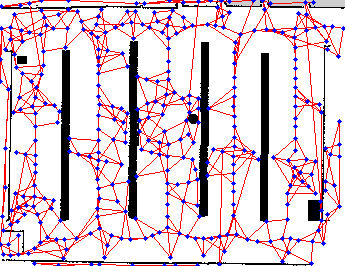
\includegraphics[width=0.8\textwidth]{voronoi_graph_V102.png}
    \caption{Final Voronoi Graph created for the environment in figure \ref{fig:gazebo_world}.}
    \label{fig:voronoi_graph3}
\end{figure}

It is now possible to verify the straight segments between the obstacles in the 
less obstacle dense areas, which allows for more efficient path planning. The denser areas 
having more nodes and edges allows for more pathing options which is useful 
for obstacle avoidance. The nodes and edges are then saved to a file to be 
then used by the planner.
\begin{figure}[h]
    \centering
    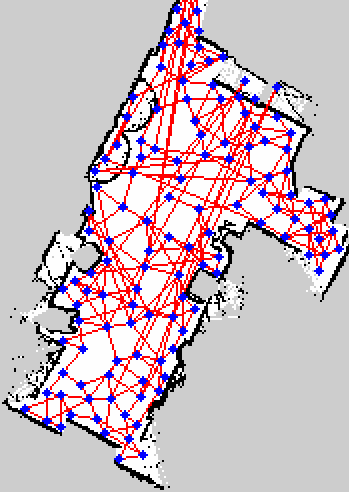
\includegraphics[width=0.9\textwidth]{basement_graph_002.png}
    \caption{Concealed room Graph.}
    \label{fig:basement_graph_002}
\end{figure}
\begin{figure}[h]
    \centering
    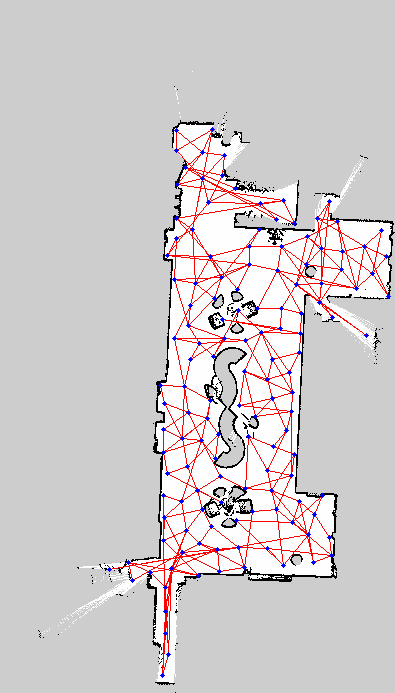
\includegraphics[width=0.85\textwidth]{corridor_graph_009.png}
    \caption{Corridor Graph.}
    \label{fig:corridor_graph_009}
\end{figure}
\clearpage

Once again, the Vorronoi Graphs aren't the usual straight line ones however, the environments 
used are not simple and have several obstacles leading to irregular graphs.

\subsection{Planner Plugin}
\label{subsec:planner_plugin}
\paragraph{}As mentioned in the subsection \ref{subsec:navigation2}, the \gls{NAV2} stack allows for the creation of custom plugins that are 
used by the different servers to perform their tasks. In this case, a custom planner plugin was 
created to be used in the Planner server, responsible for creating a global plan 
for the robot to follow. This plugin is written in C++ and uses the 
\gls{NAV2} plugin interface to be recognized by the BT Navigator server.

The plugin is responsible for the Dubins Path and Hybrid A* recovery algorithm, 
as well as the A* search algorithm that is used to find the path between the start and goal points. It is done 
by reading the file with the Voronoi Graph, verifying the closest nodes to the 
start and goal points, and then searching for the path. The resulting subpath is 
shown in figure \ref{fig:subgoals} visualized in Rviz2.
The reason this path cannot be used directly is because it is not a continuous 
smooth path, it is a set of points that serve as heuristic for the planner and 
some points could be connected in ways that are not feasible for the robot, such as reversing, and, therefore, 
a Dubins Path needs to be created.
\begin{figure}[h]
    \centering
    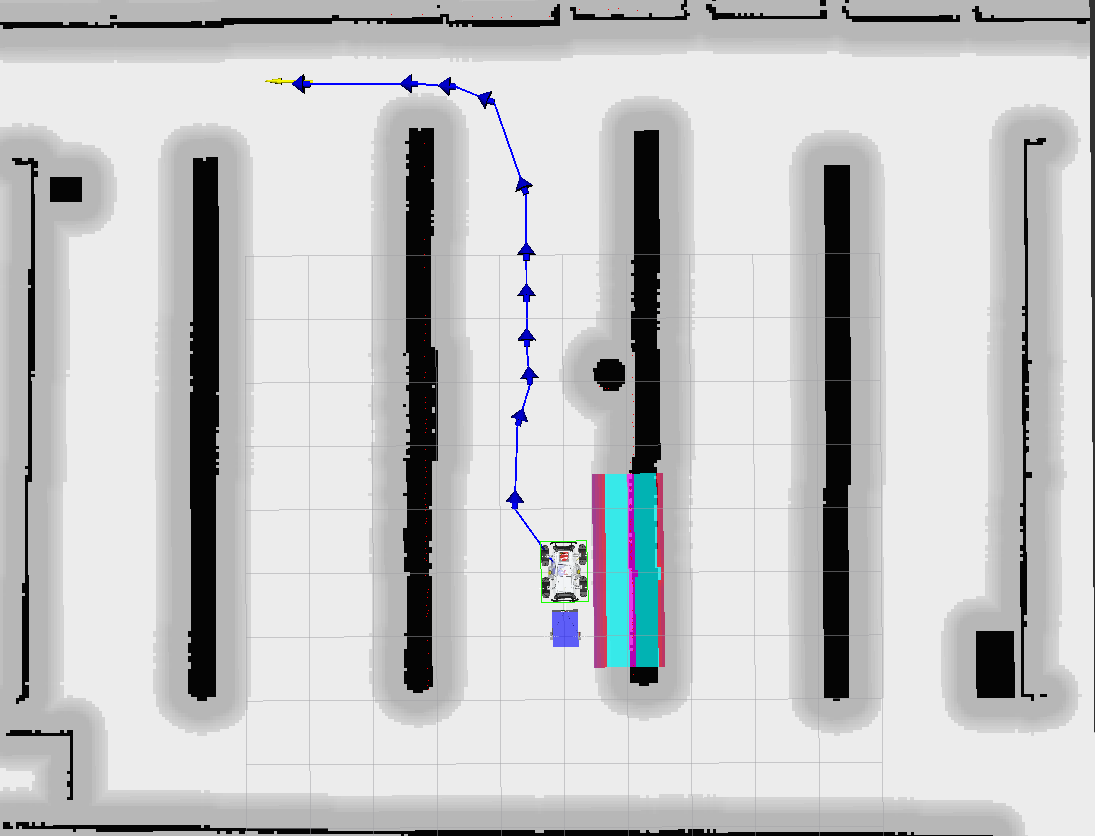
\includegraphics[width=0.9\textwidth]{subgoals.png}
    \caption{Subpath, in blue, created by the planner.}
    \label{fig:subgoals}
\end{figure}

A feature of the planner is the addition of the trailer. The planner needs to take into account 
the position of the trailer to ensure that no collisions occur while the robot is 
following the path. However, the \gls{NAV2} stack has a limitation. There's a package 
within the stack that allows for the calculation of the robot's joint values, the joint state 
publisher. This package takes in the robot's model, described in a \gls{URDF} file, and calculates the joint values 
based on the robot's movement. However this package does account for passive revolute joints, like 
the trailer connector or trailer hitch. Not accounting for this would mean 
that the trailer would either not be considered, which wouldn't make sense 
as it is the whole purpose of this robot, that the trailer would be considered 
fixed to a certain position, however this solution would not be feasible as it might make 
some curves impossible to follow, so a custom publisher was made to publish the trailer's hitch 
transform based on the trailer's movement. This publisher takes in the robot's 
dynamics defined in \ref{subsec:APP} and integrates the tractor's movement 
allowing for approximate estimation of the trailer's hitch position and orientation.


Having the trailer estimated and a rough path to follow, the nex step is to create the 
Dubins path to the desired subgoal. As explained in \ref{sec:planner1}, starting from the farthest subgoal, 
a Dubins path is created from the tractor's current position to the subgoal. Naturally, since a Dubins 
path is a collection of two curves and a straight line, the path created may not be feasible as it might 
go over obstacles or even put the trailer in undesirable positions. To check for this, with every iteration 
of the planner, the trailer position is estimated in every point of the current plan and a verification 
against jackknife conditions and obstacle collisions is performed. If any of these conditions 
are met, the Dubins path is void and a path to the next subgoal is created.

\begin{figure}[h]
    \centering
    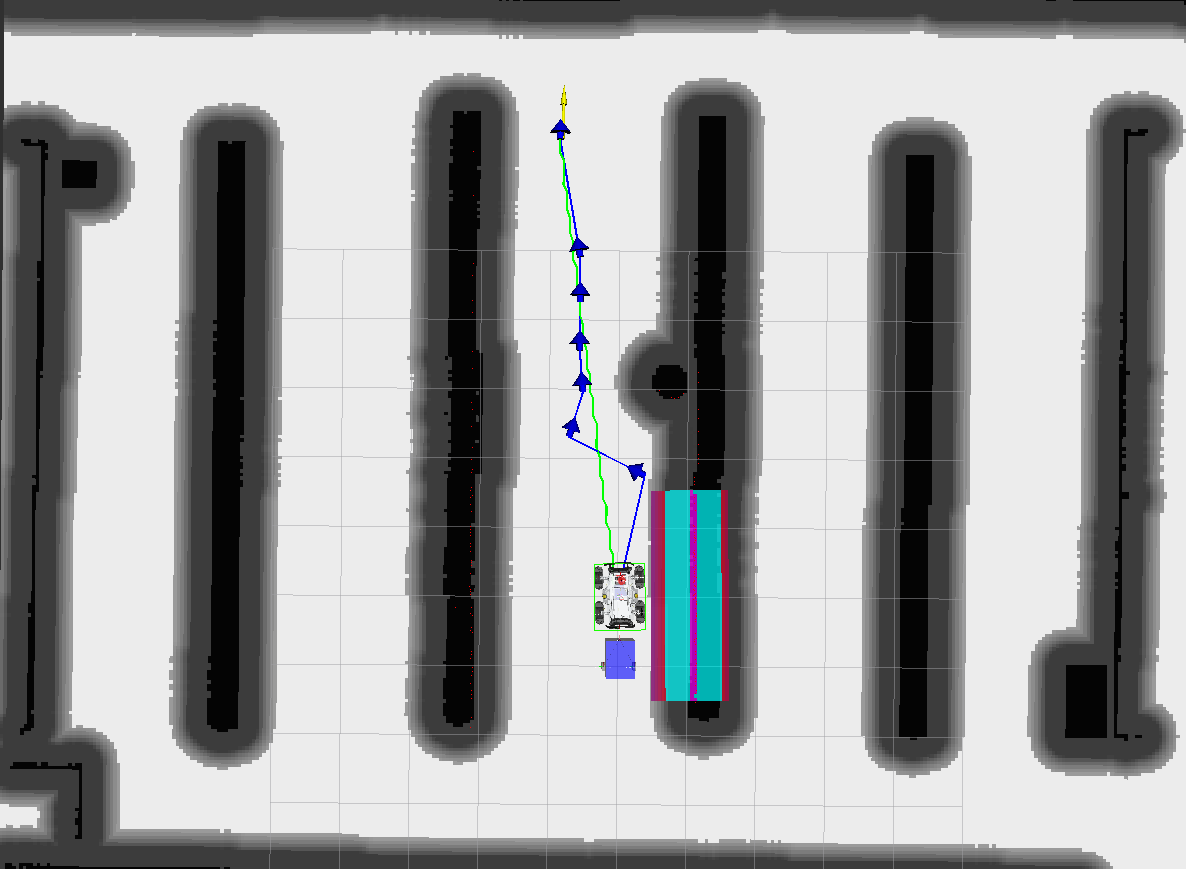
\includegraphics[width=0.9\textwidth]{dubinsonce.png}
    \caption{Dubins Path created by the planner in the first iteration.}
    \label{fig:dubins_path1}
\end{figure}
\begin{figure}[h]
    \centering
    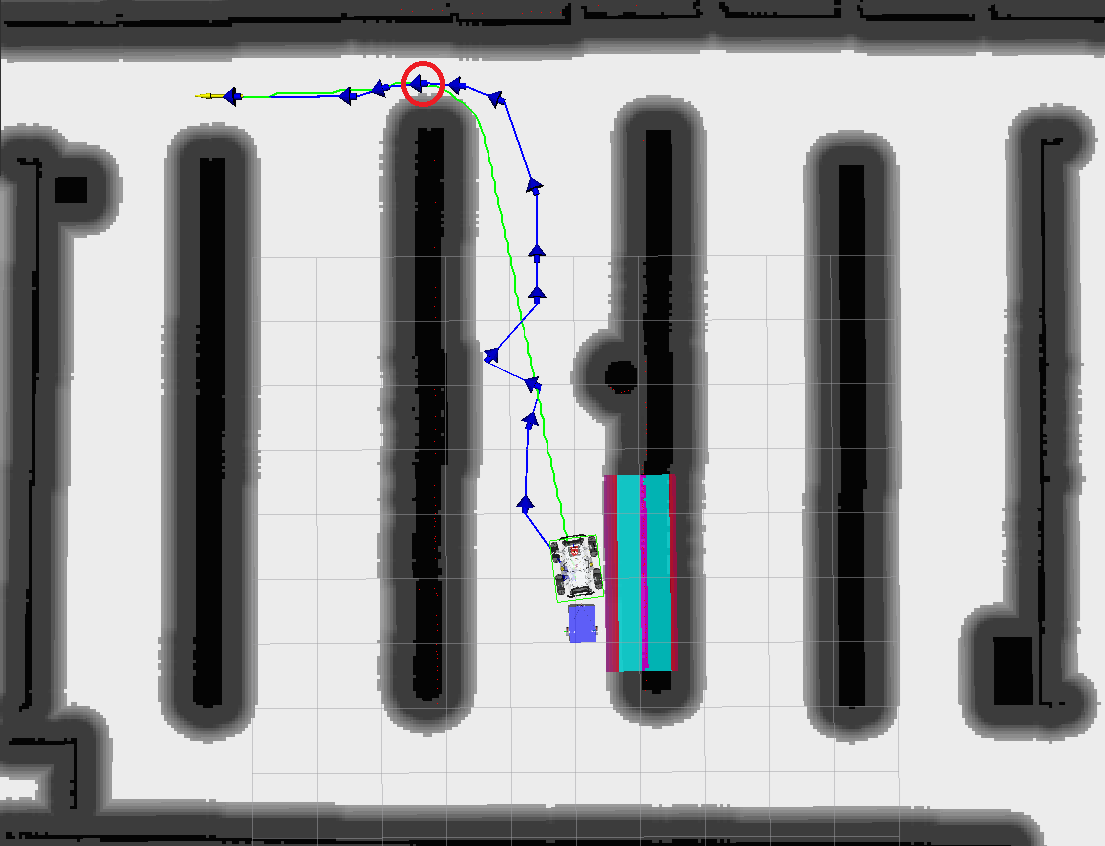
\includegraphics[width=0.8\textwidth]{dubinsmultiple.png}
    \caption{Dubins Path created by the planner in three tries. The red circle marks the subgoal used as intermediary.}
    \label{fig:dubins_path2}
\end{figure}

In picture \ref{fig:dubins_path1}, it is possible to see how the planner chooses the farthest node and tries 
to connect it to the starting position, and, since there are no obstacles or movements that would make 
the trailer jackknife, the Dubins path is valid and used. However, in picture \ref{fig:dubins_path2}, the 
planner tries to connect the tractor to the last subgoal, but cannot due to the row of crops in between 
making the planner retry three times before a suitable subgoal is found and, because the chosen subgoal 
is in clear view and aligned with the goal position, when the planner goes to repeat the algorithm 
and a direct path is found.

The last step to finish the controller is developing the recovery hybrid astar component. The previous 
examples showed how iterating through the subgoals can lead to a valid path, however, in certain cases 
it may not be the case and the loop would reach the start point without a valid path.

For these cases, a specially designed recovery module is implemented. It works by, first, reading the 
configuration file to look for the maximum angles the arcs should have. Then, it devides the maximum 
angle by the number of arcs the algorithm should have, forwards and backwards. These arcs are composed 
of a user defined number of points distanced by a user defined distance, which the last point will be 
used as a new starting point and iterate through the subgoals again.

The process of creating these arcs uses the same logic as the verification of the Dubins path for 
jackknifing, but instead of checking only for the trailer's hitch position, it checks for the tractor's 
position and orientation aswell. It is a loop iterated over the number of points starting form the starting position 
and goes one by one, calculating the next point as if the trailer was steered through the defined angle. This 
process created a number of arcs each time and can get computationally expensive if no subgoal can 
be reached over a prolonged period of time. To mitigate this, a time limit is imposed and the user will have 
to manually intervene to adjust the robot or simply set a new goal and try again.

\begin{figure}[h]
    \centering
    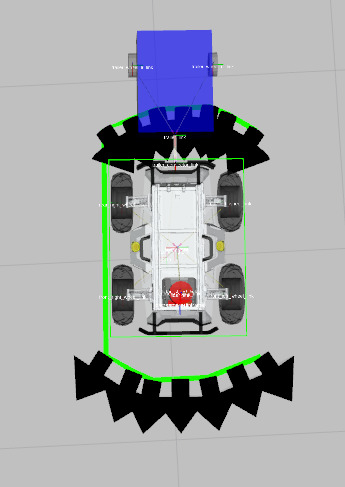
\includegraphics[width=0.3\textwidth]{Hybridastararrows.jpg}
    \caption{Hybrid A* arcs.}
    \label{fig:arrows}
\end{figure}

\begin{figure}[h]
    \centering
    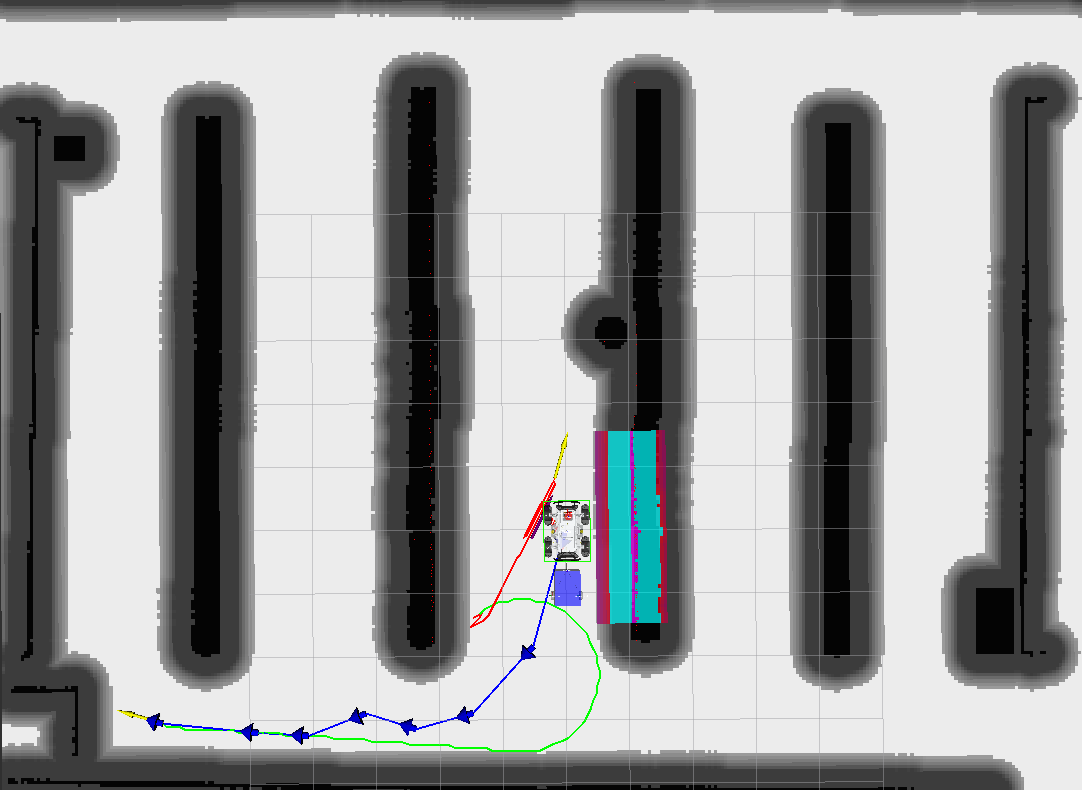
\includegraphics[width=0.8\textwidth]{hybridseg1.png}
    \caption{Successful recovery path with number of segments as one. Hybrid A* path in red, Dubins path in green, and subgoals in blue.}
    \label{fig:rseg1}
\end{figure}

At first, the number of segments was not a variable and the algorithm would always add 
one point for every iteration of the hybrid A* algorithm. This would not only worsen the computation 
time but also lead to very small adjustments in paths which could make them unfollowable by the controller, 
as shown in Figure \ref{fig:rseg1}.



\begin{figure}[h]
    \centering
    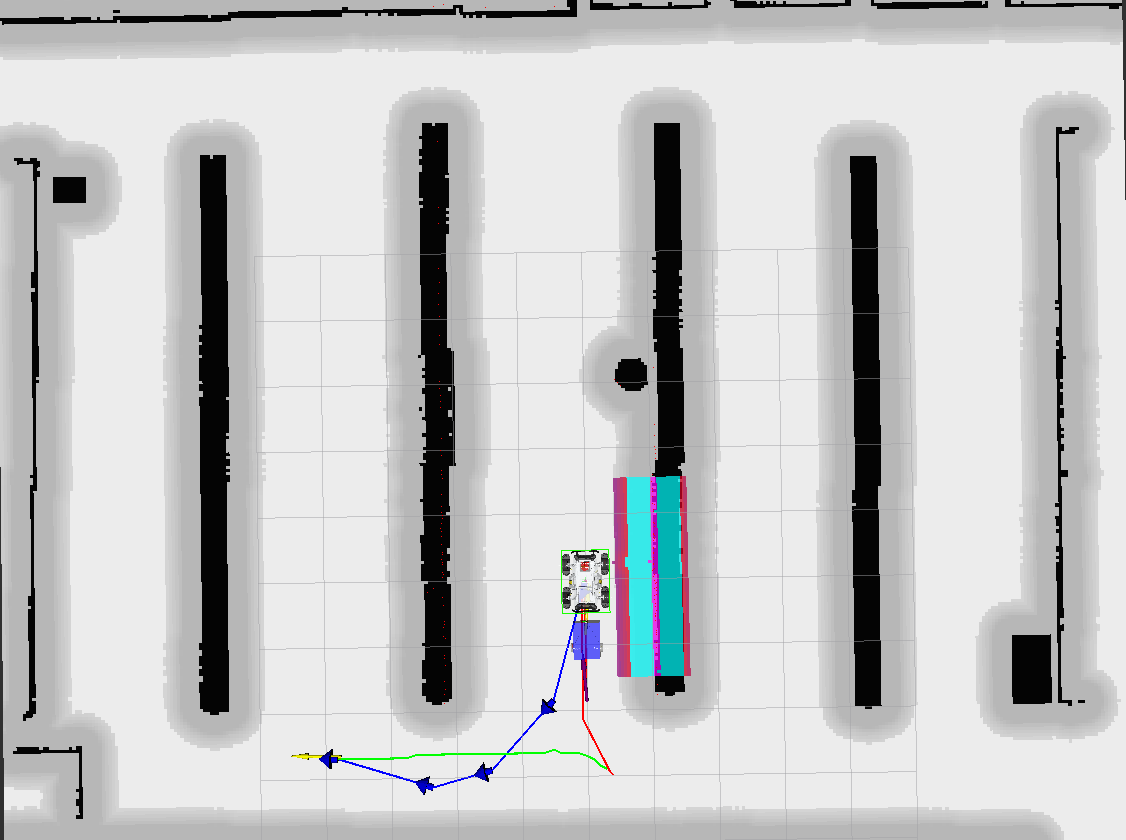
\includegraphics[width=0.8\textwidth]{hybridastarpath1.png}
    \caption{Successful recovery path with number of segments as fifteen. Hybrid A* path in red, Dubins path in green, and subgoals in blue.}
    \label{fig:recovery_module}
\end{figure}

This, of course, led to the need for the number of segments, and their length, to be a variable 
parameter and the problem was solved. The figure \ref{fig:recovery_module} shows an attempt at 
making a ninety degree turn backwards. Since the Dubins path can only find paths that make the robot move 
forwards, the hybrid A* was called and made the necessary segments to allow for the maneuvre 
to be completed successfully.

The conventional A* has the following cost function for each node:
$$f(n) = g(n) + h(n)$$
where $f(n)$ is the total cost of the node $n$, $g(n)$ is the cost to reach the node from the start node, 
and $h(n)$ is the heuristic cost to reach the goal node from the current node. However, 
in this case, since the orientation is a very important factor, it must be factored 
into the cost of each node, so the cost function is modified to:
$$f(n) = g(n) + h(n) + ap(n) + dir(n)$$
where $ap(n)$ is the angle penalty relative to the goal pose, and the $dir(n)$ 
is the direction change cost. In an initial phase the robot would be constantly making 
changes in direction going forwards and backwards multiple times, so the direction 
change cost had to be implemented to avoid unnecessary oscillations and facilitate the 
the controller's job of following the planned path.

These changes would not be enough in the end to make for efficient short hybrid path recoveries, 
and the last change made was to make the $h(n)$ cost incremental, making the cost 
of long segments too heavy to be chosen as the next node, and conditioning the 
algorithm to prefer shorter paths. The final expression was the following:
$$f(n) = g(n) + h(n) + h(n-1) + ap(n) + dir(n)$$


\section{Controller Plugin}
\label{sec:controller_plugin}
\paragraph{}The controller plugin is the component responsible for giving accurate 
velocity commands for the robot to follow the planned path. In the \gls{NAV2} stack, 
to the velocity commands have a specific type and there's only the need to change the linear 
and angular atributes of the message and return it. The controller's implementation, as a 
plugin, is similar to the planner's in the sense that it is a C++ class that 
implements the controller interface that has only a few methods that need to be implemented. 
The first method is the setPlan method. As the name suggests, this method receives the 
global plan created by the planner and stores it for when the controller may be called to 
produce velocity values. Since this controller, when in reverse, uses the trailer as the 
origin of movement, it would not make sense to have the tractor's plan as the goal 
position, therefore, when the setPlan method is called, the global plan is stored as well as 
a second plan with the trailer's position for each tractor position.

\begin{figure}[h]
    \centering
    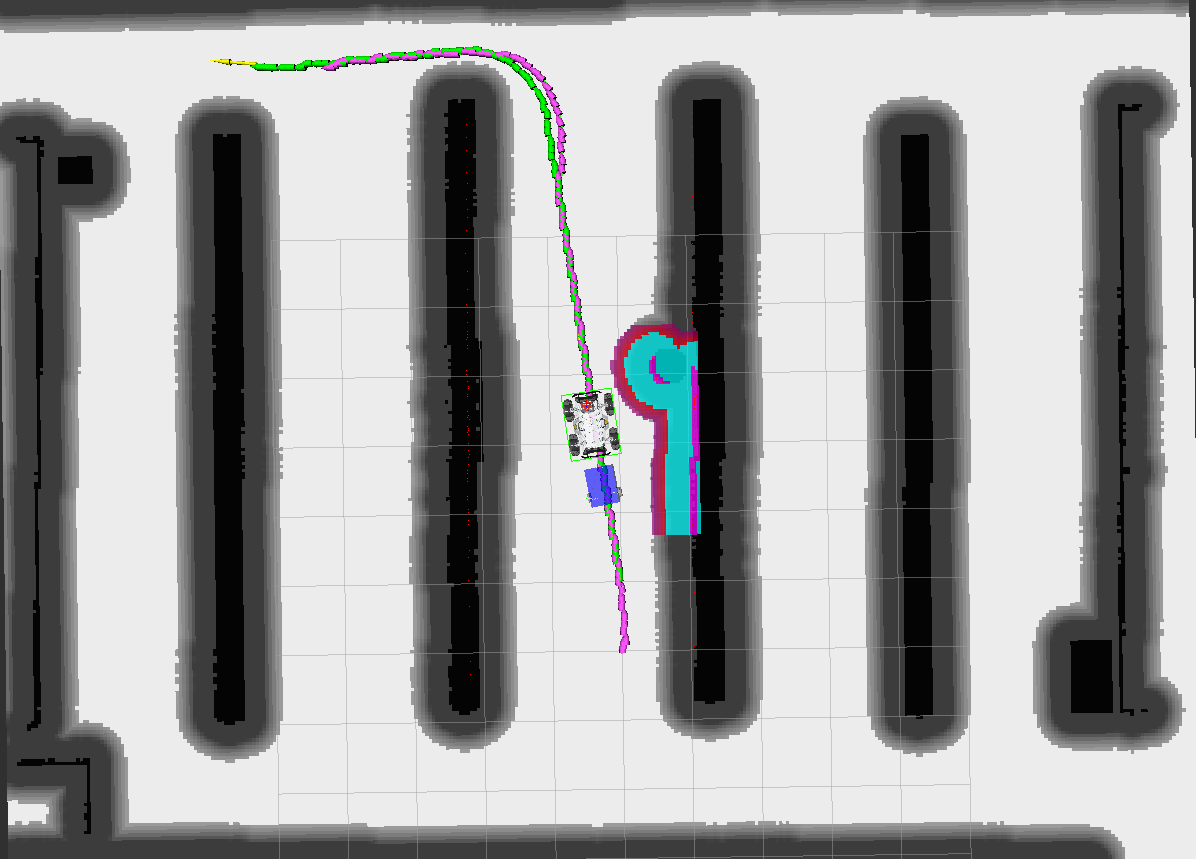
\includegraphics[width=0.8\textwidth]{trailerplan2.png}
    \caption{Trailer's positions in pink. Tractor's positions in green.}
    \label{fig:trailerplan}
\end{figure}

It is possible to observe in figure \ref{fig:trailerplan} that the trailer's 
positions are not the same as the tractor's and curve in a different maner, as the trailer 
would.

The next method is the computeVelocityCommands method. This method receives the current 
robot pose and computes the velocity values for the robot to have the desired behaviour 
for its task. Since the used controller is the pure pursuit controller, the first step is 
to compute the lookahead point in the stored path. For this, a for loop is used, starting 
from the last point used, zero if it is the first time the controller is called, and iterating 
over the points in the path until the lookahead distance is reached and the point chosen. 
If the line between the current position and the point has an angle difference of more than 
ninety degrees with the current robot heading, the robot will assume a reverse movement and 
instead of using the global path's point, the trailer's path point in the same vector position 
is used. Finally, with a constant linear velocity, changing only the sign for reversing or 
forwards movement, the angular velocity is calculated using the expressions from section 
\ref{sec:controller}, where the only adjustment made was to set the $k=2$. This value 
was chosen after some testing and it was found to be the best value for the 
controller to follow the path while ensuring that the trailer doesn't jackknife.

The collision detection was also implemented in the controller plugin as all that is 
needed for the robot to stop is to set both angular and linear velocities to zero. The 
implementation was straightforward, as explained in section \ref{sec:collision}, with the 
only caveat being that since the controller is using the local costmap for positioning, 
there was the need to create auxiliary methods to get the transform the local position to 
the global position, that is referencing the map's origin.

\section{Behaviour Tree}
\label{sec:behaviour_tree}

The original behaviour tree used by the robot calls the for a plan once per second. This is 
to ensure that the plan is always up to date with any changes in the environment and to 
correct any navigation errors that may occur. However, due to the nature of the tractor-trailer system, 
it was found that this was too frequently, as the new calculated paths would 
cause the tractor to change directions abruptly, which would lead to unwanted movement by the trailer. 
To account for this, the frequency of the planner was changed to run once every twenty seconds, 
which ensured that the tractor would follow the initial path and only change it if 
it gets in a situation where no progress is being made.